% Options for packages loaded elsewhere
\PassOptionsToPackage{unicode}{hyperref}
\PassOptionsToPackage{hyphens}{url}
%
\documentclass[
  man,floatsintext]{apa7}
\usepackage{amsmath,amssymb}
\usepackage{lmodern}
\usepackage{iftex}
\ifPDFTeX
  \usepackage[T1]{fontenc}
  \usepackage[utf8]{inputenc}
  \usepackage{textcomp} % provide euro and other symbols
\else % if luatex or xetex
  \usepackage{unicode-math}
  \defaultfontfeatures{Scale=MatchLowercase}
  \defaultfontfeatures[\rmfamily]{Ligatures=TeX,Scale=1}
\fi
% Use upquote if available, for straight quotes in verbatim environments
\IfFileExists{upquote.sty}{\usepackage{upquote}}{}
\IfFileExists{microtype.sty}{% use microtype if available
  \usepackage[]{microtype}
  \UseMicrotypeSet[protrusion]{basicmath} % disable protrusion for tt fonts
}{}
\makeatletter
\@ifundefined{KOMAClassName}{% if non-KOMA class
  \IfFileExists{parskip.sty}{%
    \usepackage{parskip}
  }{% else
    \setlength{\parindent}{0pt}
    \setlength{\parskip}{6pt plus 2pt minus 1pt}}
}{% if KOMA class
  \KOMAoptions{parskip=half}}
\makeatother
\usepackage{xcolor}
\usepackage{graphicx}
\makeatletter
\def\maxwidth{\ifdim\Gin@nat@width>\linewidth\linewidth\else\Gin@nat@width\fi}
\def\maxheight{\ifdim\Gin@nat@height>\textheight\textheight\else\Gin@nat@height\fi}
\makeatother
% Scale images if necessary, so that they will not overflow the page
% margins by default, and it is still possible to overwrite the defaults
% using explicit options in \includegraphics[width, height, ...]{}
\setkeys{Gin}{width=\maxwidth,height=\maxheight,keepaspectratio}
% Set default figure placement to htbp
\makeatletter
\def\fps@figure{htbp}
\makeatother
\setlength{\emergencystretch}{3em} % prevent overfull lines
\providecommand{\tightlist}{%
  \setlength{\itemsep}{0pt}\setlength{\parskip}{0pt}}
\setcounter{secnumdepth}{-\maxdimen} % remove section numbering
% Make \paragraph and \subparagraph free-standing
\ifx\paragraph\undefined\else
  \let\oldparagraph\paragraph
  \renewcommand{\paragraph}[1]{\oldparagraph{#1}\mbox{}}
\fi
\ifx\subparagraph\undefined\else
  \let\oldsubparagraph\subparagraph
  \renewcommand{\subparagraph}[1]{\oldsubparagraph{#1}\mbox{}}
\fi
\newlength{\cslhangindent}
\setlength{\cslhangindent}{1.5em}
\newlength{\csllabelwidth}
\setlength{\csllabelwidth}{3em}
\newlength{\cslentryspacingunit} % times entry-spacing
\setlength{\cslentryspacingunit}{\parskip}
\newenvironment{CSLReferences}[2] % #1 hanging-ident, #2 entry spacing
 {% don't indent paragraphs
  \setlength{\parindent}{0pt}
  % turn on hanging indent if param 1 is 1
  \ifodd #1
  \let\oldpar\par
  \def\par{\hangindent=\cslhangindent\oldpar}
  \fi
  % set entry spacing
  \setlength{\parskip}{#2\cslentryspacingunit}
 }%
 {}
\usepackage{calc}
\newcommand{\CSLBlock}[1]{#1\hfill\break}
\newcommand{\CSLLeftMargin}[1]{\parbox[t]{\csllabelwidth}{#1}}
\newcommand{\CSLRightInline}[1]{\parbox[t]{\linewidth - \csllabelwidth}{#1}\break}
\newcommand{\CSLIndent}[1]{\hspace{\cslhangindent}#1}
\ifLuaTeX
\usepackage[bidi=basic]{babel}
\else
\usepackage[bidi=default]{babel}
\fi
\babelprovide[main,import]{english}
% get rid of language-specific shorthands (see #6817):
\let\LanguageShortHands\languageshorthands
\def\languageshorthands#1{}
% Manuscript styling
\usepackage{upgreek}
\captionsetup{font=singlespacing,justification=justified}

% Table formatting
\usepackage{longtable}
\usepackage{lscape}
% \usepackage[counterclockwise]{rotating}   % Landscape page setup for large tables
\usepackage{multirow}		% Table styling
\usepackage{tabularx}		% Control Column width
\usepackage[flushleft]{threeparttable}	% Allows for three part tables with a specified notes section
\usepackage{threeparttablex}            % Lets threeparttable work with longtable

% Create new environments so endfloat can handle them
% \newenvironment{ltable}
%   {\begin{landscape}\centering\begin{threeparttable}}
%   {\end{threeparttable}\end{landscape}}
\newenvironment{lltable}{\begin{landscape}\centering\begin{ThreePartTable}}{\end{ThreePartTable}\end{landscape}}

% Enables adjusting longtable caption width to table width
% Solution found at http://golatex.de/longtable-mit-caption-so-breit-wie-die-tabelle-t15767.html
\makeatletter
\newcommand\LastLTentrywidth{1em}
\newlength\longtablewidth
\setlength{\longtablewidth}{1in}
\newcommand{\getlongtablewidth}{\begingroup \ifcsname LT@\roman{LT@tables}\endcsname \global\longtablewidth=0pt \renewcommand{\LT@entry}[2]{\global\advance\longtablewidth by ##2\relax\gdef\LastLTentrywidth{##2}}\@nameuse{LT@\roman{LT@tables}} \fi \endgroup}

% \setlength{\parindent}{0.5in}
% \setlength{\parskip}{0pt plus 0pt minus 0pt}

% Overwrite redefinition of paragraph and subparagraph by the default LaTeX template
% See https://github.com/crsh/papaja/issues/292
\makeatletter
\renewcommand{\paragraph}{\@startsection{paragraph}{4}{\parindent}%
  {0\baselineskip \@plus 0.2ex \@minus 0.2ex}%
  {-1em}%
  {\normalfont\normalsize\bfseries\itshape\typesectitle}}

\renewcommand{\subparagraph}[1]{\@startsection{subparagraph}{5}{1em}%
  {0\baselineskip \@plus 0.2ex \@minus 0.2ex}%
  {-\z@\relax}%
  {\normalfont\normalsize\itshape\hspace{\parindent}{#1}\textit{\addperi}}{\relax}}
\makeatother

% \usepackage{etoolbox}
\makeatletter
\patchcmd{\HyOrg@maketitle}
  {\section{\normalfont\normalsize\abstractname}}
  {\section*{\normalfont\normalsize\abstractname}}
  {}{\typeout{Failed to patch abstract.}}
\patchcmd{\HyOrg@maketitle}
  {\section{\protect\normalfont{\@title}}}
  {\section*{\protect\normalfont{\@title}}}
  {}{\typeout{Failed to patch title.}}
\makeatother

\usepackage{xpatch}
\makeatletter
\xapptocmd\appendix
  {\xapptocmd\section
    {\addcontentsline{toc}{section}{\appendixname\ifoneappendix\else~\theappendix\fi\\: #1}}
    {}{\InnerPatchFailed}%
  }
{}{\PatchFailed}
\keywords{post-error slowing, response-stimulus interval, diffusion modelling, functional account, non-functional account\newline\indent Word count: X}
\usepackage{csquotes}
\makeatletter
\renewcommand{\paragraph}{\@startsection{paragraph}{4}{\parindent}%
  {0\baselineskip \@plus 0.2ex \@minus 0.2ex}%
  {-1em}%
  {\normalfont\normalsize\bfseries\typesectitle}}

\renewcommand{\subparagraph}[1]{\@startsection{subparagraph}{5}{1em}%
  {0\baselineskip \@plus 0.2ex \@minus 0.2ex}%
  {-\z@\relax}%
  {\normalfont\normalsize\bfseries\itshape\hspace{\parindent}{#1}\textit{\addperi}}{\relax}}
\makeatother

\raggedbottom

\usepackage{hhline}

\ifLuaTeX
  \usepackage{selnolig}  % disable illegal ligatures
\fi
\IfFileExists{bookmark.sty}{\usepackage{bookmark}}{\usepackage{hyperref}}
\IfFileExists{xurl.sty}{\usepackage{xurl}}{} % add URL line breaks if available
\urlstyle{same} % disable monospaced font for URLs
\hypersetup{
  pdftitle={Effects of the Response-Stimulus-Interval on the Nature of Cognitive Processes Underlying Post-Error Slowing -- A Diffusion Model Account},
  pdfauthor={Sven Lesche1 \& Kathrin Sadus1},
  pdflang={en-EN},
  pdfkeywords={post-error slowing, response-stimulus interval, diffusion modelling, functional account, non-functional account},
  hidelinks,
  pdfcreator={LaTeX via pandoc}}

\title{Effects of the Response-Stimulus-Interval on the Nature of Cognitive Processes Underlying Post-Error Slowing -- A Diffusion Model Account}
\author{Sven Lesche\textsuperscript{1} \& Kathrin Sadus\textsuperscript{1}}
\date{}


\shorttitle{Nature of PES at Different RSI}

\authornote{

This work was completed as part of the author's bachelor-thesis.

The authors made the following contributions. Sven Lesche: Conceptualization, Writing - Original Draft Preparation, Writing - Review \& Editing; Kathrin Sadus: Supervision.

Correspondence concerning this article should be addressed to Sven Lesche, Im Neuenheimer Feld 695, 69120 Heidelberg. E-mail: \href{mailto:sven.lesche@stud.uni-heidelberg.de}{\nolinkurl{sven.lesche@stud.uni-heidelberg.de}}

}

\affiliation{\vspace{0.5cm}\textsuperscript{1} Ruprecht-Karls-University Heidelberg}

\abstract{%
One or two sentences providing a \textbf{basic introduction} to the field, comprehensible to a scientist in any discipline.

Two to three sentences of \textbf{more detailed background}, comprehensible to scientists in related disciplines.

One sentence clearly stating the \textbf{general problem} being addressed by this particular study.

One sentence summarizing the main result (with the words ``\textbf{here we show}'' or their equivalent).

Two or three sentences explaining what the \textbf{main result} reveals in direct comparison to what was thought to be the case previously, or how the main result adds to previous knowledge.

One or two sentences to put the results into a more \textbf{general context}.

Two or three sentences to provide a \textbf{broader perspective}, readily comprehensible to a scientist in any discipline.
}



\begin{document}
\maketitle

\hypertarget{introduction}{%
\section{Introduction}\label{introduction}}

``What does a man do after he makes an error?'' this title of the seminal article by Rabbitt and Rodgers (\protect\hyperlink{ref-rabbitt1977}{1977}) holds a question relevant for much of everyday life, and most certainly a question to be answered by research. The prevailing answer seems to be ``he slows down'' (e.g. \protect\hyperlink{ref-laming1968}{Laming, 1968}; \protect\hyperlink{ref-rabbitt1966a}{Rabbitt, 1966b}). This phenomenon, entering psychological literature under the name \emph{post-error slowing} (PES), describes the change in response times after subjects completing a reaction-time task commit an error (\protect\hyperlink{ref-laming1968}{Laming, 1968}, \protect\hyperlink{ref-laming1979}{1979}; \protect\hyperlink{ref-rabbitt1966a}{Rabbitt, 1966b}, \protect\hyperlink{ref-rabbitt1966b}{1966a}, \protect\hyperlink{ref-rabbitt1979}{1979}; \protect\hyperlink{ref-rabbitt1977}{Rabbitt \& Rodgers, 1977}). Average response times in trials immediately following an error are often slower than average response times in trials following a correct response. The cause of PES is still widely discussed (see \protect\hyperlink{ref-danielmeier2011}{Danielmeier \& Ullsperger, 2011} for a brief overview) and often attributed to one of two general lines of thought.

The first line of thought attributes PES to changes in information processing aiming to prevent further errors. These accounts of PES predict that error commission leads to slower response times but improved accuracy in trials following an error. Subjects that commit an error try to prevent further occurrence of errors by slowing down their response, leading to a less error-prone \emph{speed-accuracy tradeoff} (\protect\hyperlink{ref-rabbitt1979}{Rabbitt, 1979}) or by exerting cognitive control over the decision process, leading to longer but more accurate responses (\protect\hyperlink{ref-botvinick2001}{Botvinick et al., 2001}). Accounts attributing PES to cognitive processes that lead to \emph{improved} accuracy in post-error trials will henceforth be referred to as \emph{adaptive accounts} of PES.

The other line of thought claims PES to be a result of processes leading to diminished accuracy following an error. Notebaert et al. (\protect\hyperlink{ref-notebaert2009}{2009}) posit that error responses in research settings are often rarer than correct responses. The pure infrequency of an error commission then leads to an orienting response, diverting attention away from the current task and affecting performance on the trial following an infrequent error. Jentzsch and Dudschig (\protect\hyperlink{ref-jentzsch2009}{2009}) argue that given responses are always monitored for errors (see also \protect\hyperlink{ref-welford1959}{Welford, 1959}). This \emph{error-monitoring process} requires cognitive resources which cease to be available to central cognitive processes tasked with generating a response to a new stimulus. Response times on that new task will be increased if the monitoring process endures longer than the time between the potential error response and the onset of the following (post-error) trial.
Following an error, monitoring processes are more likely to impair cognitive resources otherwise directed towards the task at hand (\protect\hyperlink{ref-laming1979}{Laming, 1979}; \protect\hyperlink{ref-rabbitt1977}{Rabbitt \& Rodgers, 1977}). Responses following an error are therefore slower and less accurate. Accounts attributing PES to cognitive processes leading to \emph{reduced} accuracy in post-error trials will be referred to as \emph{maladaptive accounts} of PES.

Adaptive and maladaptive accounts of PES both posit an increase in response time in trials following an error but seem to be at odds regarding the accuracy of post-error trials. Support for adaptive accounts of PES comes from behavioral data (\protect\hyperlink{ref-laming1979}{Laming, 1979}; \protect\hyperlink{ref-mooji2021}{Mooij et al., 2021}; \protect\hyperlink{ref-steinhauser2017}{Steinhauser et al., 2017}), mathematical models of cognitive processes (\protect\hyperlink{ref-dutilh2012testing}{Dutilh et al., 2012}; \protect\hyperlink{ref-schiffler2017}{Schiffler et al., 2017}) and neurophysiological research using electroencephalography (EEG) (\protect\hyperlink{ref-carp2009}{Carp \& Compton, 2009}; \protect\hyperlink{ref-saunders2012}{Saunders \& Jentzsch, 2012}). Conversely, a variety of studies show behavioral decreases in accuracy following errors (\protect\hyperlink{ref-dali2022error}{Dali et al., 2022}; \protect\hyperlink{ref-dudschig2009}{Dudschig \& Jentzsch, 2009}; \protect\hyperlink{ref-houtman2013}{Houtman \& Notebaert, 2013}; \protect\hyperlink{ref-jentzsch2009}{Jentzsch \& Dudschig, 2009}; \protect\hyperlink{ref-vanderborght2016errors}{Van der Borght et al., 2016}) or following infrequent events more generally (\protect\hyperlink{ref-castellar2010}{Castellar et al., 2010}; \protect\hyperlink{ref-notebaert2009}{Notebaert et al., 2009}). Further support for maladaptive accounts can be found in studies showing impaired cognitive processes as measured via EEG (\protect\hyperlink{ref-buzzel2017}{Buzzell et al., 2017}; \protect\hyperlink{ref-vanderborght2016errors}{Van der Borght et al., 2016}) or as mapped by mathematical models of reaction time (\protect\hyperlink{ref-dutilh2013}{Dutilh et al., 2013}; \protect\hyperlink{ref-purcell2016}{Purcell \& Kiani, 2016}; \protect\hyperlink{ref-schiffler2017}{Schiffler et al., 2017}).

Intrigued by the diversity of findings regarding the functionality of PES, Jentzsch and Dudschig (\protect\hyperlink{ref-jentzsch2009}{2009}) identified a key variable moderating the influence of processes deemed adaptive or maladaptive -- the response-stimulus interval (RSI). Depending on the time between a subject's response to trial \emph{n} and the onset of trial \emph{n+1}, Jentzsch and Dudschig were able to observe different patterns of accuracy changes following an error. When the RSI was long (1000ms), errors led to increased response times and a slight increase in accuracy, lending support to adaptive accounts of PES. Was the RSI short (50ms) on the other hand, the same increase in response times was paired with a decrease in accuracy, a finding supporting maladaptive accounts. The same pattern of shorter RSI leading to decreases in accuracy, while longer RSI led to increases or significantly smaller accuracy losses was replicated for four different levels of RSI (\protect\hyperlink{ref-dudschig2009}{Dudschig \& Jentzsch, 2009}). The time between an error response and the onset of the trial following it thus influences whether patterns supporting adaptive or maladaptive accounts are found.

Even though adaptive and maladaptive accounts postulate different cognitive processes underlying PES, these explanations are not necessarily mutually exclusive (\protect\hyperlink{ref-danielmeier2011}{Danielmeier \& Ullsperger, 2011}; \protect\hyperlink{ref-schiffler2017}{Schiffler et al., 2017}; \protect\hyperlink{ref-steinhauser2017}{Steinhauser et al., 2017}). Depending on trial timing, specifically the onset of trial \emph{n+1} following an error, different cognitive processes may influence response timing. Error-monitoring processes only impair response time and accuracy if they last longer than the RSI. Should the error-monitoring process of trial \emph{n} come to a conclusion prior to the start of trial \emph{n+1}, central cognitive resources are fully available to be dedicated to responding to trial \emph{n+1} (\protect\hyperlink{ref-dudschig2009}{Dudschig \& Jentzsch, 2009}; \protect\hyperlink{ref-jentzsch2009}{Jentzsch \& Dudschig, 2009}). Similarly, orienting responses following the infrequent appearance of an error are deemed to only divert attention away from the task for a short period of time, after which the subject refocuses on the task at hand (\protect\hyperlink{ref-notebaert2009}{Notebaert et al., 2009}). Cognitive processes hypothesized to be responsible for PES by adaptive accounts, such as increased cognitive control being recruited after an error, take some amount of time before they can influence information processing (\protect\hyperlink{ref-botvinick2001}{Botvinick et al., 2001}). Adaptive changes to information processing thus exert more control over response times of trial \emph{n+1} at long RSI than at short RSI. Depending on the RSI between trial \emph{n} in which an error is committed and trial \emph{n+1}, different cognitive processes underlie PES (\protect\hyperlink{ref-ullsperger2016}{Ullsperger \& Danielmeier, 2016}).

Buzzell et al. (\protect\hyperlink{ref-buzzel2017}{2017}) employed the use of an electroencephalogram (EEG) to examine cognitive processes responsible for PES at different RSI. Changes in certain components of \emph{event related potentials} (ERP), specifically reduced P1 amplitude following an error, reflect attentional deficits leading to impaired sensory processing. Reduced P1 amplitude was however only observed at short RSI. At long RSI these deficits are not present, indicating support for the time-specificity of attentional deficits elicited by errors.

The present study will make use of \emph{evidence accumulation models} (EAM) more specifically the \emph{drift diffusion model} (DDM) (\protect\hyperlink{ref-ratcliff1978}{Ratcliff, 1978}) to investigate cognitive processes underlying behavior in reaction-time tasks. EAM enable mapping model parameters to specific cognitive processes responsible for response-behavior of each subject (\protect\hyperlink{ref-dutilh2012testing}{Dutilh et al., 2012}; \protect\hyperlink{ref-voss2004}{Voss et al., 2004}).
Behavioral data can then be accounted for by multiple model parameters each carrying information about cognitive processes underlying a subject's responses.

In order to be comparable to previous research on PES using EAM (\protect\hyperlink{ref-dutilh2012testing}{Dutilh et al., 2012}, \protect\hyperlink{ref-dutilh2013}{2013}; \protect\hyperlink{ref-purcell2016}{Purcell \& Kiani, 2016}; \protect\hyperlink{ref-schiffler2017}{Schiffler et al., 2017}), this study will focus on modeling response data using the DDM. Recent publications have however pointed to potential issues arising with fitting DDM to PES data and have suggested using \emph{linear ballistic accumulator} (LBA) modeling to avoid misfits (\protect\hyperlink{ref-damaso2022}{Damaso et al., 2022}). Future research will aim to compare DDM and LBA fitted to behavioral data and further investigate possible benefits and drawbacks of each mode of analysis. To reduce the scope of this body of work, all EAM analysis will be conducted using the DDM.



\begin{figure}
\centering
\includegraphics{images/ddm-slide/Slide1.png}
\caption{\label{fig:ddm-slide}Ratcliff-Drift-Diffusion Model}
\end{figure}

The standard DDM for two-choice tasks assumes a noisy accumulation of pieces of evidence supporting one of two response alternatives. Once the accumulated amount of evidence pointing towards one of the response alternatives reaches a certain threshold, a response is given. Several different parameters guide this process. First, response time is separated into decision time, where the noisy evidence accumulation process takes place, and non-decision time \emph{T\textsubscript{er}}. Non-decision time incorporates processes such as stimulus encoding and motor processes. Decision time is further controlled by three main parameters: (1) boundary separation \emph{a} describes the distance between decision thresholds and represents the amount of evidence required to reach a decision, (2) mean drift rate \emph{v} is the average rate at which evidence is accumulated and (3) mean starting point \emph{z} represents the average point at which, with some potential a-priori bias towards one of the two-choice alternatives, the evidence accumulation process begins. Further parameters of across-trial variability are added to reflect changes in diffusion model parameters over time. Variability of the starting point \emph{s\textsubscript{z}} accounts for differences in a-priori bias towards one response alternative across trials (\protect\hyperlink{ref-laming1968}{Laming, 1968}; \protect\hyperlink{ref-ratcliff1998}{Ratcliff \& Rouder, 1998}). Variability of drift rate \(\eta\) reflects changes in drift rate across trials and allows the model to account for systematic differences between trials, such as error responses being systematically faster than correct responses (\protect\hyperlink{ref-ratcliff1978}{Ratcliff, 1978}; \protect\hyperlink{ref-ratcliff1998}{Ratcliff \& Rouder, 1998}). Finally, variability of non-decision time \emph{s\textsubscript{t}} reflects fluctuations in the duration of encoding or motor-execution processes across trials.

Dutilh et al. (\protect\hyperlink{ref-dutilh2012testing}{2012}) outlined several explanations of PES and the respective parameters in the DDM that would be able to reflect these accounts. The aim of their study was to investigate which of the different accounts find greatest support in diffusion model analysis of their data. Dutilh et al.~investigated support for five different accounts of PES, each mapping to a change in one parameter of the DDM. Since no studies to date have supported accounts corresponding to a shift in starting point \emph{z} or decreased variability \emph{s\textsubscript{z}} following an error, only three of the five mappings will be discussed further here.

\begin{enumerate}
\def\labelenumi{(\arabic{enumi})}
\tightlist
\item
  Delayed startup of evidence accumulation following an error response (\protect\hyperlink{ref-rabbitt1977}{Rabbitt \& Rodgers, 1977}) finds reflection in longer non-decision time \emph{T\textsubscript{er}} on trials following an error. Increases in \emph{T\textsubscript{er}} were able to account for PES in a random dot motion task (\protect\hyperlink{ref-dutilh2013}{Dutilh et al., 2013}). While not directly affecting accuracy and thus not being strictly attributable to either adaptive or maladaptive accounts of PES, the only account predicting increases in \emph{T\textsubscript{er}} is the lag induced by longer \emph{error monitoring processes} (\protect\hyperlink{ref-dudschig2009}{Dudschig \& Jentzsch, 2009}; \protect\hyperlink{ref-jentzsch2009}{Jentzsch \& Dudschig, 2009}).
\item
  Distraction of attention leading to impaired evidence accumulation, caused by an orienting response (\protect\hyperlink{ref-notebaert2009}{Notebaert et al., 2009}) or diminished cognitive resources due to error-monitoring processes (\protect\hyperlink{ref-dudschig2009}{Dudschig \& Jentzsch, 2009}; \protect\hyperlink{ref-jentzsch2009}{Jentzsch \& Dudschig, 2009}) leads to lower drift rates \emph{v} following an error. Lowered drift rates in post-error trials compared to pre-error trials were found in multiple tasks (\protect\hyperlink{ref-dutilh2013}{Dutilh et al., 2013}; \protect\hyperlink{ref-purcell2016}{Purcell \& Kiani, 2016}; \protect\hyperlink{ref-schiffler2017}{Schiffler et al., 2017}).
\item
  An increase in boundary separation \emph{a} corresponds to increased caution when responding after an error. Changes in \emph{a} are predicted by the cognitive control account of PES (\protect\hyperlink{ref-botvinick2001}{Botvinick et al., 2001}). Following an error, cognitive control is exerted in order to prevent occurrence of future errors. Heightened caution is reflected in a larger amount of evidence needed to reach a decision. An increase in \emph{a} was able to predict PES in a range of studies (\protect\hyperlink{ref-dutilh2012testing}{Dutilh et al., 2012}; \protect\hyperlink{ref-purcell2016}{Purcell \& Kiani, 2016}; \protect\hyperlink{ref-schiffler2017}{Schiffler et al., 2017}).
\end{enumerate}

Dutilh et al. (\protect\hyperlink{ref-dutilh2012testing}{2012}) found increases in boundary separation \emph{a} following error trials to be responsible for PES, increases in \emph{T\textsubscript{er}} or decreases in \emph{v} were not supported by evidence. The authors interpret their findings as support for adaptive accounts of PES. Critically, the RSI (500ms) was of medium length and not as short as RSI leading to increases in the influence of maladaptive processes found in previous studies (\protect\hyperlink{ref-buzzel2017}{Buzzell et al., 2017}; \protect\hyperlink{ref-dudschig2009}{Dudschig \& Jentzsch, 2009}; \protect\hyperlink{ref-jentzsch2009}{Jentzsch \& Dudschig, 2009}). Realizing a shorter RSI trial-condition might generate results lending more support maladaptive accounts. No study to date has fitted a DDM to data with RSI~\(< 300ms\) or systematically manipulated the RSI within participants to evaluate parameter shifts responsible for PES. The present study will attempt to fill this gap in research.

Our aim is to evaluate the effects of different RSI on the nature of cognitive processes causing PES. To achieve this goal, we will realize two RSI conditions with respective lengths commonly used for short and long intervals. A Drift Diffusion Model will be fit to data in both conditions, allowing further dissection of cognitive processes underlying subjects' responses. Changes in DDM parameters between pre-error and post-error trials will be analysed for each RSI condition. According to theory outlined above, differential influences of adaptive/maladaptive processes at different RSI should lead to respective differences in changes in DDM parameters following an error trial. When the RSI is long, changes in DDM parameters leading to slower post-error response times (PES) should be mostly attributable to parameters linked to increased accuracy, such as an increased \emph{boundary separation}. Changes in parameters reflecting attentional deficits, such as a decreased \emph{drift rate} should account for PES at shorter RSI.

\hypertarget{method}{%
\section{Method}\label{method}}

\hypertarget{power-analysis}{%
\subsection{Power analysis}\label{power-analysis}}

We conducted a power analysis using the the R package \texttt{superpower} (\protect\hyperlink{ref-R-Superpower}{Lakens \& Caldwell, 2021}) with values based on previous studies (\protect\hyperlink{ref-dutilh2012testing}{Dutilh et al., 2012}, \protect\hyperlink{ref-dutilh2013}{2013}) to determine the minimum sample size needed to detect an interaction effect of RSI and \emph{trial type} (pre- vs.~post-error) on drift rate and boundary separation. Mean values for each cell were entered into the model to estimate effect sizes, returning interaction effects of partial \(\eta^2 =\) 0.11 and 0.17 for effects on drift rate and boundary separation, respectively. Using bonferroni corrected significance criteria of \(\alpha\) = 0.02 and power \(= .80\), minimum sample size required to detect the hypothesized interaction effects was estimated to be N = 49 for effects on boundary separation and N = 84 for effects on drift rate. Exact values entered into analysis can be found in Table \ref{tab:mean-values-power-analysis} in the appendix.

\hypertarget{participants}{%
\subsection{Participants}\label{participants}}

In order to account for potential exclusion of participants and to \textbf{somewhat combat the effects of testing multiple ANOVA (alpha-cummulation)} we collected \textbf{NUMBER OF PARTICIPANTS}

\hypertarget{materials}{%
\subsection{Materials}\label{materials}}

The experiment was programmed using the PsychoPy software (\protect\hyperlink{ref-peirce2019}{Peirce et al., 2019}). We used a modified version of the Behavior Adaptation Task (BAT) (\protect\hyperlink{ref-hester2007}{Hester et al., 2007}) -- a motor-inhibition Go-NoGo task. Stimuli consisted of a stream of the letters X and Y presented centrally on a grey background. Subjects were asked to respond to the letters when they occurred in an alternating pattern (Go-trial) but withhold their response on repeated presentation of a stimulus (NoGo-trial).
Instructions on response mappings of stimuli X and Y to the response keys D and L were counterbalanced across participants. Only errors in NoGo-trials were considered \emph{error trials} used for further analysis in order decrease variance of processes leading to an error. \textbf{this isn't quite right, is it? Why don't I use other errors?}



\begin{figure}
\centering
\includegraphics{images/bat_slide_pp/Slide1.png}
\caption{\label{fig:bat-example}Behavioral Adaptation Task}
\end{figure}

\hypertarget{procedure}{%
\subsection{Procedure}\label{procedure}}

Participants were asked to respond as quickly and accurately as possible. Stimuli were presented for 800ms or until a response was given. We set the RSI to 200ms for the short condition and 1000ms for the long condition. A fixation cross was presented during the RSI period. Participants completed 30 practice trials, 15 of which with short RSI and 15 with long RSI. Participants only received feedback informing them about their performance in practice trials. RSI was manipulated between experimental blocks, with six blocks consisting of 250 trials each being presented per RSI condition. Blocks of short and long RSI occurred in an alternating pattern, beginning with the long RSI condition. A self-paced break was administered following each experimental block. \textbf{instruction screens (german) can be found in supplementary materials?)} The sequence of appearance of stimuli X and Y was generated pseudo-randomly. Fourfold repetitions of a stimulus were prohibited, and NoGo-trials were always preceded by another NoGo-trial or at least two Go-trials. This was done to ensure that post-error trials were never simultaneously pre-error trials.

\hypertarget{data-analysis}{%
\subsection{Data analysis}\label{data-analysis}}

\begin{itemize}
\tightlist
\item
  with what programs were models fit?
\item
  how was PES measured (robust classification)
\end{itemize}

Analysis was conducted using R (Version 4.1.1; \protect\hyperlink{ref-R-base}{R Core Team, 2021}) and the R-packages \emph{papaja} (Version 0.1.1.9001; \protect\hyperlink{ref-R-papaja}{Aust \& Barth, 2022}), and \emph{tidyverse} (Version 1.3.1; \protect\hyperlink{ref-R-tidyverse}{Wickham et al., 2019}).

\hypertarget{outline-method}{%
\subsection{Outline Method}\label{outline-method}}

\begin{itemize}
\tightlist
\item
  Introduce Task used
\item
  explain modifications and expectations
\item
  stimuli, procedure\ldots{}
\item
  describe participants
\item
  describe analysis model used (check convention when DDM is introduced)
\item
  describe the procedure of analysis
\end{itemize}

\hypertarget{results}{%
\section{Results}\label{results}}

\hypertarget{outline-results}{%
\subsection{Outline Results}\label{outline-results}}

\begin{itemize}
\tightlist
\item
  data included
\item
  outliers and data excluded
\item
  behavioral description of effects
\item
  replicate pes, check interaction RSI and so forth
\item
  diffusion modelling things
\item
  describe differential effects of errors on parameters in RSI conditions
\end{itemize}

\hypertarget{trying-data-insertation}{%
\subsection{Trying data insertation}\label{trying-data-insertation}}

\begin{table}

\caption{\label{tab:display}some data}
\centering
\begin{tabular}[t]{r|r|r|r}
\hline
first & second & third & fourth\\
\hline
1 & 1 & 1 & 1\\
\hline
2 & 2 & 2 & 2\\
\hline
3 & 3 & 3 & 3\\
\hline
4 & 4 & 4 & 4\\
\hline
5 & 5 & 5 & 5\\
\hline
\end{tabular}
\end{table}

\hypertarget{discussion}{%
\section{Discussion}\label{discussion}}

\hypertarget{outline-discussion}{%
\subsection{Outline Discussion}\label{outline-discussion}}

\begin{itemize}
\tightlist
\item
  give basic overview of hypothesis
\item
  describe the task and analysis procedure
\item
  review important findings of current study
\item
  check theoretical implications (find anything of interest)?
\item
  describe importance of this body of research
\item
  limitations: task-used, DDM model can't fit this? stimuli generation usw.
\item
  \textbf{can already discuss some of the limitations!}
\end{itemize}

\newpage

\hypertarget{references}{%
\section{References}\label{references}}

\hypertarget{refs}{}
\begin{CSLReferences}{1}{0}
\leavevmode\vadjust pre{\hypertarget{ref-R-papaja}{}}%
Aust, F., \& Barth, M. (2022). \emph{{papaja}: {Prepare} reproducible {APA} journal articles with {R Markdown}}. \url{https://github.com/crsh/papaja}

\leavevmode\vadjust pre{\hypertarget{ref-botvinick2001}{}}%
Botvinick, M. M., Braver, T. S., Barch, D. M., Carter, C. S., \& Cohen, J. D. (2001). Conflict monitoring and cognitive control {[}Journal Article{]}. \emph{Psychological Review}, \emph{108}(3), 624--652. \url{https://doi.org/10.1037/0033-295X.108.3.624}

\leavevmode\vadjust pre{\hypertarget{ref-buzzel2017}{}}%
Buzzell, G. A., Beatty, P. J., Paquette, N. A., Roberts, D. M., \& McDonald, C. G. (2017). Error-induced blindness: Error detection leads to impaired sensory processing and lower accuracy at short response--stimulus intervals {[}Journal Article{]}. \emph{Journal of Neuroscience}, \emph{37}(11), 2895--2903.

\leavevmode\vadjust pre{\hypertarget{ref-carp2009}{}}%
Carp, J., \& Compton, R. J. (2009). Alpha power is influenced by performance errors {[}Journal Article{]}. \emph{Psychophysiology}, \emph{46}(2), 336--343. \url{https://doi.org/10.1111/j.1469-8986.2008.00773.x}

\leavevmode\vadjust pre{\hypertarget{ref-castellar2010}{}}%
Castellar, E. N., Kühn, S., Fias, W., \& Notebaert, W. (2010). Outcome expectancy and not accuracy determines posterror slowing: ERP support {[}Journal Article{]}. \emph{Cognitive, Affective, \& Behavioral Neuroscience}, \emph{10}(2), 270--278. \url{https://doi.org/10.3758/cabn.10.2.270}

\leavevmode\vadjust pre{\hypertarget{ref-dali2022error}{}}%
Dali, G., Orr, C., \& Hester, R. (2022). Error awareness and post-error slowing: The effect of manipulating trial intervals {[}Journal Article{]}. \emph{Consciousness and Cognition}, \emph{98}, 103282. \url{https://doi.org/10.1016/j.concog.2022.103282}

\leavevmode\vadjust pre{\hypertarget{ref-damaso2022}{}}%
Damaso, K. A. M., Williams, P. G., \& Heathcote, A. (2022). What happens after a fast versus slow error, and how does it relate to evidence accumulation? {[}Journal Article{]}. \emph{Computational Brain \& Behavior}. \url{https://doi.org/10.1007/s42113-022-00137-2}

\leavevmode\vadjust pre{\hypertarget{ref-danielmeier2011}{}}%
Danielmeier, C., \& Ullsperger, M. (2011). Post-error adjustments {[}Journal Article{]}. \emph{Frontiers in Psychology}, \emph{2}. \url{https://doi.org/10.3389/fpsyg.2011.00233}

\leavevmode\vadjust pre{\hypertarget{ref-dudschig2009}{}}%
Dudschig, C., \& Jentzsch, I. (2009). Speeding before and slowing after errors: Is it all just strategy? {[}Journal Article{]}. \emph{Brain Research}, \emph{1296}, 56--62. \url{https://doi.org/10.1016/j.brainres.2009.08.009}

\leavevmode\vadjust pre{\hypertarget{ref-dutilh2013}{}}%
Dutilh, G., Forstmann, B. U., Vandekerckhove, J., \& Wagenmakers, E.-J. (2013). A diffusion model account of age differences in posterror slowing {[}Journal Article{]}. \emph{Psychology and Aging}, \emph{28}(1), 64--76. \url{https://doi.org/10.1037/a0029875}

\leavevmode\vadjust pre{\hypertarget{ref-dutilh2012testing}{}}%
Dutilh, G., Vandekerckhove, J., Forstmann, B. U., Keuleers, E., Brysbaert, M., \& Wagenmakers, E.-J. (2012). Testing theories of post-error slowing {[}Journal Article{]}. \emph{Attention, Perception, \& Psychophysics}, \emph{74}(2), 454--465. \url{https://doi.org/10.3758/s13414-011-0243-2}

\leavevmode\vadjust pre{\hypertarget{ref-hester2007}{}}%
Hester, R., Simões-Franklin, C., \& Garavan, H. (2007). Post-error behavior in active cocaine users: Poor awareness of errors in the presence of intact performance adjustments {[}Journal Article{]}. \emph{Neuropsychopharmacology}, \emph{32}(9), 1974--1984. \url{https://doi.org/10.1038/sj.npp.1301326}

\leavevmode\vadjust pre{\hypertarget{ref-houtman2013}{}}%
Houtman, F., \& Notebaert, W. (2013). Blinded by an error {[}Journal Article{]}. \emph{Cognition}, \emph{128}(2), 228--236. \url{https://doi.org/10.1016/j.cognition.2013.04.003}

\leavevmode\vadjust pre{\hypertarget{ref-jentzsch2009}{}}%
Jentzsch, I., \& Dudschig, C. (2009). Short article: Why do we slow down after an error? Mechanisms underlying the effects of posterror slowing {[}Journal Article{]}. \emph{Quarterly Journal of Experimental Psychology}, \emph{62}(2), 209--218. \url{https://doi.org/10.1080/17470210802240655}

\leavevmode\vadjust pre{\hypertarget{ref-R-Superpower}{}}%
Lakens, D., \& Caldwell, A. (2021). Simulation-based power analysis for factorial analysis of variance designs. \emph{Advances in Methods and Practices in Psychological Science}, \emph{4}(1), 251524592095150. \url{https://doi.org/10.1177/2515245920951503}

\leavevmode\vadjust pre{\hypertarget{ref-laming1968}{}}%
Laming, D. (1968). \emph{Information theory of choice-reaction times} {[}Book{]}. Academic Press.

\leavevmode\vadjust pre{\hypertarget{ref-laming1979}{}}%
Laming, D. (1979). Choice reaction performance following an error {[}Journal Article{]}. \emph{Acta Psychologica}, \emph{43}(3), 199--224. \url{https://doi.org/10.1016/0001-6918(79)90026-X}

\leavevmode\vadjust pre{\hypertarget{ref-mooji2021}{}}%
Mooij, S. M. M., Dumontheil, I., Kirkham, N. Z., Raijmakers, M. E. J., \& Maas, H. L. J. (2021). Post‐error slowing: Large scale study in an online learning environment for practising mathematics and language {[}Journal Article{]}. \emph{Developmental Science}. \url{https://doi.org/10.1111/desc.13174}

\leavevmode\vadjust pre{\hypertarget{ref-notebaert2009}{}}%
Notebaert, W., Houtman, F., Van Opstal, F., Gevers, W., Fias, W., \& Verguts, T. (2009). Post-error slowing: An orienting account {[}Journal Article{]}. \emph{Cognition}, \emph{111}(2), 275--279. \url{https://doi.org/10.1016/j.cognition.2009.02.002}

\leavevmode\vadjust pre{\hypertarget{ref-peirce2019}{}}%
Peirce, J., Gray, J. R., Simpson, S., Macaskill, M., Höchenberger, R., Sogo, H., Kastman, E., \& Lindeløv, J. K. (2019). PsychoPy2: Experiments in behavior made easy {[}Journal Article{]}. \emph{Behavior Research Methods}, \emph{51}(1), 195--203. \url{https://doi.org/10.3758/s13428-018-01193-y}

\leavevmode\vadjust pre{\hypertarget{ref-purcell2016}{}}%
Purcell, B., \& Kiani, R. (2016). Neural mechanisms of post-error adjustments of decision policy in parietal cortex {[}Journal Article{]}. \emph{Neuron}, \emph{89}(3), 658--671. \url{https://doi.org/10.1016/j.neuron.2015.12.027}

\leavevmode\vadjust pre{\hypertarget{ref-R-base}{}}%
R Core Team. (2021). \emph{R: A language and environment for statistical computing}. R Foundation for Statistical Computing. \url{https://www.R-project.org/}

\leavevmode\vadjust pre{\hypertarget{ref-rabbitt1966b}{}}%
Rabbitt, P. (1966a). Error correction time without external error signals {[}Journal Article{]}. \emph{Nature}, \emph{212}(5060), 438--438. \url{https://doi.org/10.1038/212438a0}

\leavevmode\vadjust pre{\hypertarget{ref-rabbitt1966a}{}}%
Rabbitt, P. (1966b). Errors and error correction in choice-response tasks {[}Journal Article{]}. \emph{Journal of Experimental Psychology}, \emph{71}(2), 264--272. \url{https://doi.org/10.1037/h0022853}

\leavevmode\vadjust pre{\hypertarget{ref-rabbitt1979}{}}%
Rabbitt, P. (1979). How old and young subjects monitor and control responses for accuracy and speed {[}Journal Article{]}. \emph{British Journal of Psychology}, \emph{70}(2), 305--311. \url{https://doi.org/10.1111/j.2044-8295.1979.tb01687.x}

\leavevmode\vadjust pre{\hypertarget{ref-rabbitt1977}{}}%
Rabbitt, P., \& Rodgers, B. (1977). What does a man do after he makes an error? An analysis of response programming {[}Journal Article{]}. \emph{Quarterly Journal of Experimental Psychology}, \emph{29}(4), 727--743. \url{https://doi.org/10.1080/14640747708400645}

\leavevmode\vadjust pre{\hypertarget{ref-ratcliff1978}{}}%
Ratcliff, R. (1978). A theory of memory retrieval {[}Journal Article{]}. \emph{Psychological Review}, \emph{85}(2), 59.

\leavevmode\vadjust pre{\hypertarget{ref-ratcliff1998}{}}%
Ratcliff, R., \& Rouder, J. N. (1998). Modeling response times for two-choice decisions {[}Journal Article{]}. \emph{Psychological Science}, \emph{9}(5), 347--356. \url{https://doi.org/10.1111/1467-9280.00067}

\leavevmode\vadjust pre{\hypertarget{ref-saunders2012}{}}%
Saunders, B., \& Jentzsch, I. (2012). False external feedback modulates posterror slowing and the f-P300: Implications for theories of posterror adjustment {[}Journal Article{]}. \emph{Psychonomic Bulletin \& Review}, \emph{19}(6), 1210--1216. \url{https://doi.org/10.3758/s13423-012-0314-y}

\leavevmode\vadjust pre{\hypertarget{ref-schiffler2017}{}}%
Schiffler, B. C., Bengtsson, S. L., \& Lundqvist, D. (2017). The sustained influence of an error on future decision-making {[}Journal Article{]}. \emph{Frontiers in Psychology}, \emph{8}. \url{https://doi.org/10.3389/fpsyg.2017.01077}

\leavevmode\vadjust pre{\hypertarget{ref-steinhauser2017}{}}%
Steinhauser, M., Ernst, B., \& Ibald, K. W. (2017). Isolating component processes of posterror slowing with the psychological refractory period paradigm {[}Journal Article{]}. \emph{Journal of Experimental Psychology: Learning, Memory, and Cognition}, \emph{43}(4), 653--659. \url{https://doi.org/10.1037/xlm0000329}

\leavevmode\vadjust pre{\hypertarget{ref-ullsperger2016}{}}%
Ullsperger, M., \& Danielmeier, C. (2016). Reducing speed and sight: How adaptive is post-error slowing? {[}Journal Article{]}. \emph{Neuron}, \emph{89}(3), 430--432. \url{https://doi.org/10.1016/j.neuron.2016.01.035}

\leavevmode\vadjust pre{\hypertarget{ref-vanderborght2016errors}{}}%
Van der Borght, L., Schevernels, H., Burle, B., \& Notebaert, W. (2016). Errors disrupt subsequent early attentional processes {[}Journal Article{]}. \emph{PLOS ONE}, \emph{11}(4), e0151843. \url{https://doi.org/10.1371/journal.pone.0151843}

\leavevmode\vadjust pre{\hypertarget{ref-voss2004}{}}%
Voss, A., Rothermund, K., \& Voss, J. (2004). Interpreting the parameters of the diffusion model: An empirical validation {[}Journal Article{]}. \emph{Memory \& Cognition}, \emph{32}(7), 1206--1220. \url{https://doi.org/10.3758/bf03196893}

\leavevmode\vadjust pre{\hypertarget{ref-welford1959}{}}%
Welford, A. (1959). Evidence of a single-channel decision mechanism limiting performance in a serial reaction task {[}Journal Article{]}. \emph{Quarterly Journal of Experimental Psychology}, \emph{11}(4), 193--210.

\leavevmode\vadjust pre{\hypertarget{ref-R-tidyverse}{}}%
Wickham, H., Averick, M., Bryan, J., Chang, W., McGowan, L. D., François, R., Grolemund, G., Hayes, A., Henry, L., Hester, J., Kuhn, M., Pedersen, T. L., Miller, E., Bache, S. M., Müller, K., Ooms, J., Robinson, D., Seidel, D. P., Spinu, V., \ldots{} Yutani, H. (2019). Welcome to the {tidyverse}. \emph{Journal of Open Source Software}, \emph{4}(43), 1686. \url{https://doi.org/10.21105/joss.01686}

\end{CSLReferences}

\newpage

\hypertarget{appendix}{%
\section{Appendix}\label{appendix}}

\begin{table}

\providecommand{\docline}[3]{\noalign{\global\setlength{\arrayrulewidth}{#1}}\arrayrulecolor[HTML]{#2}\cline{#3}}

\setlength{\tabcolsep}{0pt}

\renewcommand*{\arraystretch}{1.5}

\begin{longtable}[l]{|p{1.58in}|p{0.75in}|p{0.83in}|p{0.89in}|p{0.83in}|p{0.89in}}

\caption{Mean\ values\ and\ standard\ deviations\ used\ for\ power\ analysis}\label{tab:mean-values-power-analysis}\\

\hhline{>{\arrayrulecolor[HTML]{000000}\global\arrayrulewidth=1pt}->{\arrayrulecolor[HTML]{000000}\global\arrayrulewidth=1pt}->{\arrayrulecolor[HTML]{000000}\global\arrayrulewidth=1pt}->{\arrayrulecolor[HTML]{000000}\global\arrayrulewidth=1pt}->{\arrayrulecolor[HTML]{000000}\global\arrayrulewidth=1pt}->{\arrayrulecolor[HTML]{000000}\global\arrayrulewidth=1pt}-}

\multicolumn{1}{!{\color[HTML]{000000}\vrule width 0pt}>{\centering}p{\dimexpr 1.58in+0\tabcolsep+0\arrayrulewidth}}{} & \multicolumn{1}{!{\color[HTML]{000000}\vrule width 0pt}>{\centering}p{\dimexpr 0.75in+0\tabcolsep+0\arrayrulewidth}}{} & \multicolumn{2}{!{\color[HTML]{000000}\vrule width 0pt}>{\centering}p{\dimexpr 1.72in+2\tabcolsep+1\arrayrulewidth}}{\textcolor[HTML]{000000}{\fontsize{11}{22}\selectfont{Short\ RSI}}} & \multicolumn{2}{!{\color[HTML]{000000}\vrule width 0pt}>{\centering}p{\dimexpr 1.72in+2\tabcolsep+1\arrayrulewidth}!{\color[HTML]{000000}\vrule width 0pt}}{\textcolor[HTML]{000000}{\fontsize{11}{22}\selectfont{Long\ RSI}}} \\

\hhline{~~>{\arrayrulecolor[HTML]{666666}\global\arrayrulewidth=1pt}->{\arrayrulecolor[HTML]{666666}\global\arrayrulewidth=1pt}->{\arrayrulecolor[HTML]{666666}\global\arrayrulewidth=1pt}->{\arrayrulecolor[HTML]{666666}\global\arrayrulewidth=1pt}-}



\multicolumn{1}{!{\color[HTML]{000000}\vrule width 0pt}>{\centering}p{\dimexpr 1.58in+0\tabcolsep+0\arrayrulewidth}}{\multirow[c]{-2}{*}{\parbox{1.58in}{\textcolor[HTML]{000000}{\fontsize{11}{22}\selectfont{Parameter}}}}} & \multicolumn{1}{!{\color[HTML]{000000}\vrule width 0pt}>{\centering}p{\dimexpr 0.75in+0\tabcolsep+0\arrayrulewidth}}{\multirow[c]{-2}{*}{\parbox{0.75in}{\textcolor[HTML]{000000}{\fontsize{11}{22}\selectfont{\ }}}}} & \multicolumn{1}{!{\color[HTML]{000000}\vrule width 0pt}>{\centering}p{\dimexpr 0.83in+0\tabcolsep+0\arrayrulewidth}}{\textcolor[HTML]{000000}{\fontsize{11}{22}\selectfont{pre-error}}} & \multicolumn{1}{!{\color[HTML]{000000}\vrule width 0pt}>{\centering}p{\dimexpr 0.89in+0\tabcolsep+0\arrayrulewidth}}{\textcolor[HTML]{000000}{\fontsize{11}{22}\selectfont{post-error}}} & \multicolumn{1}{!{\color[HTML]{000000}\vrule width 0pt}>{\centering}p{\dimexpr 0.83in+0\tabcolsep+0\arrayrulewidth}}{\textcolor[HTML]{000000}{\fontsize{11}{22}\selectfont{pre-error}}} & \multicolumn{1}{!{\color[HTML]{000000}\vrule width 0pt}>{\centering}p{\dimexpr 0.89in+0\tabcolsep+0\arrayrulewidth}!{\color[HTML]{000000}\vrule width 0pt}}{\textcolor[HTML]{000000}{\fontsize{11}{22}\selectfont{post-error}}} \\

\hhline{>{\arrayrulecolor[HTML]{000000}\global\arrayrulewidth=1pt}->{\arrayrulecolor[HTML]{000000}\global\arrayrulewidth=1pt}->{\arrayrulecolor[HTML]{000000}\global\arrayrulewidth=1pt}->{\arrayrulecolor[HTML]{000000}\global\arrayrulewidth=1pt}->{\arrayrulecolor[HTML]{000000}\global\arrayrulewidth=1pt}->{\arrayrulecolor[HTML]{000000}\global\arrayrulewidth=1pt}-}\endhead



\multicolumn{1}{!{\color[HTML]{000000}\vrule width 0pt}>{\raggedright}p{\dimexpr 1.58in+0\tabcolsep+0\arrayrulewidth}}{\textcolor[HTML]{000000}{\fontsize{11}{22}\selectfont{Drift\ Rate}}} & \multicolumn{1}{!{\color[HTML]{000000}\vrule width 0pt}>{\centering}p{\dimexpr 0.75in+0\tabcolsep+0\arrayrulewidth}}{\textcolor[HTML]{000000}{\fontsize{11}{22}\selectfont{}}} & \multicolumn{1}{!{\color[HTML]{000000}\vrule width 0pt}>{\centering}p{\dimexpr 0.83in+0\tabcolsep+0\arrayrulewidth}}{\textcolor[HTML]{000000}{\fontsize{11}{22}\selectfont{}}} & \multicolumn{1}{!{\color[HTML]{000000}\vrule width 0pt}>{\centering}p{\dimexpr 0.89in+0\tabcolsep+0\arrayrulewidth}}{\textcolor[HTML]{000000}{\fontsize{11}{22}\selectfont{}}} & \multicolumn{1}{!{\color[HTML]{000000}\vrule width 0pt}>{\centering}p{\dimexpr 0.83in+0\tabcolsep+0\arrayrulewidth}}{\textcolor[HTML]{000000}{\fontsize{11}{22}\selectfont{}}} & \multicolumn{1}{!{\color[HTML]{000000}\vrule width 0pt}>{\centering}p{\dimexpr 0.89in+0\tabcolsep+0\arrayrulewidth}!{\color[HTML]{000000}\vrule width 0pt}}{\textcolor[HTML]{000000}{\fontsize{11}{22}\selectfont{}}} \\





\multicolumn{1}{!{\color[HTML]{000000}\vrule width 0pt}>{\raggedright}p{\dimexpr 1.58in+0\tabcolsep+0\arrayrulewidth}}{\textcolor[HTML]{000000}{\fontsize{11}{22}\selectfont{}}} & \multicolumn{1}{!{\color[HTML]{000000}\vrule width 0pt}>{\centering}p{\dimexpr 0.75in+0\tabcolsep+0\arrayrulewidth}}{\textcolor[HTML]{000000}{\fontsize{11}{22}\selectfont{Mean}}} & \multicolumn{1}{!{\color[HTML]{000000}\vrule width 0pt}>{\centering}p{\dimexpr 0.83in+0\tabcolsep+0\arrayrulewidth}}{\textcolor[HTML]{000000}{\fontsize{11}{22}\selectfont{0.230}}} & \multicolumn{1}{!{\color[HTML]{000000}\vrule width 0pt}>{\centering}p{\dimexpr 0.89in+0\tabcolsep+0\arrayrulewidth}}{\textcolor[HTML]{000000}{\fontsize{11}{22}\selectfont{0.180}}} & \multicolumn{1}{!{\color[HTML]{000000}\vrule width 0pt}>{\centering}p{\dimexpr 0.83in+0\tabcolsep+0\arrayrulewidth}}{\textcolor[HTML]{000000}{\fontsize{11}{22}\selectfont{0.240}}} & \multicolumn{1}{!{\color[HTML]{000000}\vrule width 0pt}>{\centering}p{\dimexpr 0.89in+0\tabcolsep+0\arrayrulewidth}!{\color[HTML]{000000}\vrule width 0pt}}{\textcolor[HTML]{000000}{\fontsize{11}{22}\selectfont{0.220}}} \\





\multicolumn{1}{!{\color[HTML]{000000}\vrule width 0pt}>{\raggedright}p{\dimexpr 1.58in+0\tabcolsep+0\arrayrulewidth}}{\textcolor[HTML]{000000}{\fontsize{11}{22}\selectfont{}}} & \multicolumn{1}{!{\color[HTML]{000000}\vrule width 0pt}>{\centering}p{\dimexpr 0.75in+0\tabcolsep+0\arrayrulewidth}}{\textcolor[HTML]{000000}{\fontsize{11}{22}\selectfont{SD}}} & \multicolumn{1}{!{\color[HTML]{000000}\vrule width 0pt}>{\centering}p{\dimexpr 0.83in+0\tabcolsep+0\arrayrulewidth}}{\textcolor[HTML]{000000}{\fontsize{11}{22}\selectfont{0.080}}} & \multicolumn{1}{!{\color[HTML]{000000}\vrule width 0pt}>{\centering}p{\dimexpr 0.89in+0\tabcolsep+0\arrayrulewidth}}{\textcolor[HTML]{000000}{\fontsize{11}{22}\selectfont{0.080}}} & \multicolumn{1}{!{\color[HTML]{000000}\vrule width 0pt}>{\centering}p{\dimexpr 0.83in+0\tabcolsep+0\arrayrulewidth}}{\textcolor[HTML]{000000}{\fontsize{11}{22}\selectfont{0.080}}} & \multicolumn{1}{!{\color[HTML]{000000}\vrule width 0pt}>{\centering}p{\dimexpr 0.89in+0\tabcolsep+0\arrayrulewidth}!{\color[HTML]{000000}\vrule width 0pt}}{\textcolor[HTML]{000000}{\fontsize{11}{22}\selectfont{0.080}}} \\





\multicolumn{1}{!{\color[HTML]{000000}\vrule width 0pt}>{\raggedright}p{\dimexpr 1.58in+0\tabcolsep+0\arrayrulewidth}}{\textcolor[HTML]{000000}{\fontsize{11}{22}\selectfont{Boundary\ Separation}}} & \multicolumn{1}{!{\color[HTML]{000000}\vrule width 0pt}>{\centering}p{\dimexpr 0.75in+0\tabcolsep+0\arrayrulewidth}}{\textcolor[HTML]{000000}{\fontsize{11}{22}\selectfont{}}} & \multicolumn{1}{!{\color[HTML]{000000}\vrule width 0pt}>{\centering}p{\dimexpr 0.83in+0\tabcolsep+0\arrayrulewidth}}{\textcolor[HTML]{000000}{\fontsize{11}{22}\selectfont{}}} & \multicolumn{1}{!{\color[HTML]{000000}\vrule width 0pt}>{\centering}p{\dimexpr 0.89in+0\tabcolsep+0\arrayrulewidth}}{\textcolor[HTML]{000000}{\fontsize{11}{22}\selectfont{}}} & \multicolumn{1}{!{\color[HTML]{000000}\vrule width 0pt}>{\centering}p{\dimexpr 0.83in+0\tabcolsep+0\arrayrulewidth}}{\textcolor[HTML]{000000}{\fontsize{11}{22}\selectfont{}}} & \multicolumn{1}{!{\color[HTML]{000000}\vrule width 0pt}>{\centering}p{\dimexpr 0.89in+0\tabcolsep+0\arrayrulewidth}!{\color[HTML]{000000}\vrule width 0pt}}{\textcolor[HTML]{000000}{\fontsize{11}{22}\selectfont{}}} \\





\multicolumn{1}{!{\color[HTML]{000000}\vrule width 0pt}>{\raggedright}p{\dimexpr 1.58in+0\tabcolsep+0\arrayrulewidth}}{\textcolor[HTML]{000000}{\fontsize{11}{22}\selectfont{}}} & \multicolumn{1}{!{\color[HTML]{000000}\vrule width 0pt}>{\centering}p{\dimexpr 0.75in+0\tabcolsep+0\arrayrulewidth}}{\textcolor[HTML]{000000}{\fontsize{11}{22}\selectfont{Mean}}} & \multicolumn{1}{!{\color[HTML]{000000}\vrule width 0pt}>{\centering}p{\dimexpr 0.83in+0\tabcolsep+0\arrayrulewidth}}{\textcolor[HTML]{000000}{\fontsize{11}{22}\selectfont{0.120}}} & \multicolumn{1}{!{\color[HTML]{000000}\vrule width 0pt}>{\centering}p{\dimexpr 0.89in+0\tabcolsep+0\arrayrulewidth}}{\textcolor[HTML]{000000}{\fontsize{11}{22}\selectfont{0.135}}} & \multicolumn{1}{!{\color[HTML]{000000}\vrule width 0pt}>{\centering}p{\dimexpr 0.83in+0\tabcolsep+0\arrayrulewidth}}{\textcolor[HTML]{000000}{\fontsize{11}{22}\selectfont{0.130}}} & \multicolumn{1}{!{\color[HTML]{000000}\vrule width 0pt}>{\centering}p{\dimexpr 0.89in+0\tabcolsep+0\arrayrulewidth}!{\color[HTML]{000000}\vrule width 0pt}}{\textcolor[HTML]{000000}{\fontsize{11}{22}\selectfont{0.155}}} \\





\multicolumn{1}{!{\color[HTML]{000000}\vrule width 0pt}>{\raggedright}p{\dimexpr 1.58in+0\tabcolsep+0\arrayrulewidth}}{\textcolor[HTML]{000000}{\fontsize{11}{22}\selectfont{}}} & \multicolumn{1}{!{\color[HTML]{000000}\vrule width 0pt}>{\centering}p{\dimexpr 0.75in+0\tabcolsep+0\arrayrulewidth}}{\textcolor[HTML]{000000}{\fontsize{11}{22}\selectfont{SD}}} & \multicolumn{1}{!{\color[HTML]{000000}\vrule width 0pt}>{\centering}p{\dimexpr 0.83in+0\tabcolsep+0\arrayrulewidth}}{\textcolor[HTML]{000000}{\fontsize{11}{22}\selectfont{0.020}}} & \multicolumn{1}{!{\color[HTML]{000000}\vrule width 0pt}>{\centering}p{\dimexpr 0.89in+0\tabcolsep+0\arrayrulewidth}}{\textcolor[HTML]{000000}{\fontsize{11}{22}\selectfont{0.020}}} & \multicolumn{1}{!{\color[HTML]{000000}\vrule width 0pt}>{\centering}p{\dimexpr 0.83in+0\tabcolsep+0\arrayrulewidth}}{\textcolor[HTML]{000000}{\fontsize{11}{22}\selectfont{0.020}}} & \multicolumn{1}{!{\color[HTML]{000000}\vrule width 0pt}>{\centering}p{\dimexpr 0.89in+0\tabcolsep+0\arrayrulewidth}!{\color[HTML]{000000}\vrule width 0pt}}{\textcolor[HTML]{000000}{\fontsize{11}{22}\selectfont{0.020}}} \\

\hhline{>{\arrayrulecolor[HTML]{000000}\global\arrayrulewidth=1pt}->{\arrayrulecolor[HTML]{000000}\global\arrayrulewidth=1pt}->{\arrayrulecolor[HTML]{000000}\global\arrayrulewidth=1pt}->{\arrayrulecolor[HTML]{000000}\global\arrayrulewidth=1pt}->{\arrayrulecolor[HTML]{000000}\global\arrayrulewidth=1pt}->{\arrayrulecolor[HTML]{000000}\global\arrayrulewidth=1pt}-}



\multicolumn{6}{!{\color[HTML]{FFFFFF}\vrule width 0pt}>{\raggedright}p{\dimexpr 5.76in+10\tabcolsep+5\arrayrulewidth}!{\color[HTML]{FFFFFF}\vrule width 0pt}}{\textcolor[HTML]{000000}{\fontsize{11}{22}\selectfont{\textit{Note.\ }}}\textcolor[HTML]{000000}{\fontsize{11}{22}\selectfont{Values\ based\ on\ previous\ research\ by\ Dutilh\ et\ al.\ (2012,\ 2013).}}} \\





\end{longtable}

\end{table}


\end{document}
